\documentclass[tikz,border=10pt]{standalone}
\usepackage{amsmath}
\usepackage{mathrsfs}

\begin{document}

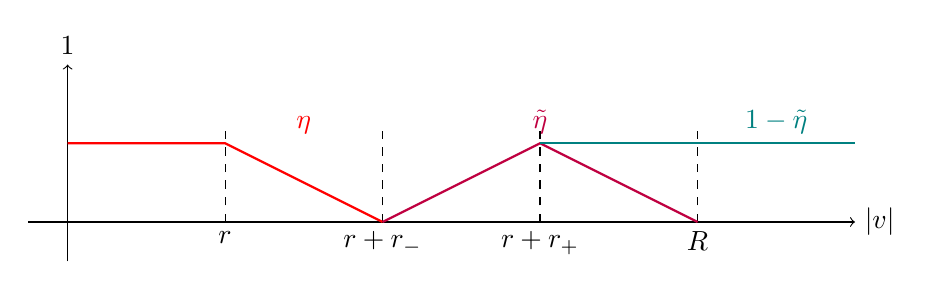
\begin{tikzpicture}
    % Axis
    \draw[->] (-0.5,0) -- (10,0) node[right] {$|v|$};
    \draw[->] (0,-0.5) -- (0,2) node[above] {$1$};

    % Dashed lines and labels
    \draw[dashed] (2,0) -- (2,1.2);
    \draw[dashed] (4,0) -- (4,1.2);
    \draw[dashed] (6,0) -- (6,1.2);
    \draw[dashed] (8,0) -- (8,1.2);

    \node[below] at (2,0) {$r$};
    \node[below] at (4,0) {$r + r_-$};
    \node[below] at (6,0) {$r + r_+$};
    \node[below] at (8,0) {$R$};

    % Plotting the lines for eta, tilde eta, and 1-tilde eta
    \draw[thick, red] (0,1) -- (2,1) -- (4,0);
    \node[red, above] at (3,1) {$\eta$};

    \draw[thick, purple] (4,0) -- (6,1) -- (8,0);
    \node[purple, above] at (6,1) {$\tilde{\eta}$};

    \draw[thick, teal] (6,1) -- (8,1) -- (10,1);
    \node[teal, above] at (9,1) {$1-\tilde{\eta}$};
\end{tikzpicture}

\end{document}